%% Einleitung
\section{Einleitung}
\label{sec1:intro}
Die Digitalisierung der Welt schreitet immer rasanter voran. Nicht zuletzt wird im Kontext der Digitalisierung auch von dem \enquote{Informationszeitalter} und \enquote{Computerisierung} gesprochen \cite{gabler-digitalisierung}.
In einer zunehmend digitalen Welt nimmt die Anzahl internetfähiger digitaler Geräte, den sogenannten \textit{Internet Of Things} (IoT)-Geräten und Anwendern derselben immer mehr zu \cite{statista-iot-devices}.
Laut Statistiken belief sich die Zahl der Internetnutzer, den sogenannten \enquote{Onlinern} \cite{statista-onliner-2022}, im Jahr 2022 auf rund 5.3 Milliarden.
Im Vergleich zum letzten Jahrzehnt ist somit die Anzahl der Internetanwender innerhalb eines Jahrzehnts um rund 2.9 Milliarden auf beinahe das Doppelte angestiegen \cite{statista-onliner-2022}.
Auch die weltweite \textit{Covid-19}-Pandemie hatte keinen hindernden Effekt auf diese Entwicklung \cite{mckinsey-digitalization-covid}.
Aufgrund der Pandemie waren viele Menschen dazu gezwungen, mehr Zeit zu Hause zu verbringen, oder von zu Hause aus zu arbeiten.
Dies hatte zur Folge, dass mehr Menschen sich digitalen Technologien und Lösungen zuwandten, um mittels Videokonferenzsystemen von zu Hause aus zu arbeiten, oder mittels sozialer Medien mit Freunden und Bekannten in Kontakt zu bleiben \cite{mckinsey-digitalization-covid, statista-covid-social-media-use}.
Anhand der weltweiten Reaktionen auf die Pandemie wurde die Umstellung auf digitale Technologien um mehrere Jahre beschleunigt \cite{mckinsey-digitalization-covid}.
Die Verwendung dieser Technologien, wie z.B. den sozialen Medien, wie Instagram \cite{instagram}, Facebook \cite{facebook}, Snapchat \cite{snapchat} und weiteren, führt zu enormen Datenmengen, die ohne Hilfsmittel für Menschen nicht mehr greifbar und überschaubar sind.
So betrug die Datennutzung im Jahr 2022 schätzungsweise 100 000 Petabytes, von welchem Mobiltelefone einen Großteil ausmachten \cite{global-mobile-data-usage}.

Sollen, unabhängig vom Anwendungsbereich, diese enormen Datenmengen und die daraus extrahierten Merkmale effektiv verarbeitet, und gewonnene Erkenntnisse effektiv kommuniziert werden, so gilt es, die Beziehung zwischen der Darstellung der identifizierten Merkmale und der für Menschen verständlichen Bedeutung zu berücksichtigen.
Zwischen der Darstellung der identifizierten Merkmale und der für Menschen verständlichen Bedeutung besteht eine sogenannte semantische Lücke, die es zu überbrücken gilt \cite{bridging-semantic-gap}.
Die semantische Lücke bezeichnet hierbei den Unterschied zwischen den jeweiligen Darstellungsformen.
Die Darstellungsform der identifizierten Merkmale ist ihre maschinelle Darstellung in Form von Nullen und Einsen, auch binäre Darstellung genannt, und die Darstellung der für Menschen verständliche Bedeutung kann in natürlicher Sprache erfolgen.
Zwischen diesen Darstellungsformen liegt eine semantische Lücke, dessen Überbrückung in dieser Arbeit untersucht werden soll.
Das Überbrücken dieser semantischen Lücke ist eine große Herausforderung und wird seit Jahren intensiv erforscht und ist, aufgrund immer breiterer Anwendung, Gegenstand zahlreicher Untersuchungen im Bereich des \mmiri{} \cite{bridging-semantic-gap}.

\clearpage

Das Thema dieser Arbeit ist im Bereich \mmir{} und künstlicher Intelligenz (KI) verortet.
Das Themengebiet der künstlichen Intelligenz ist nicht neu und schon seit Jahrzehnten Gegenstand der Forschung und zahlreicher Untersuchungen \cite{harvard-history-ai-research}.
Die Anwendungsmöglichkeiten von künstlicher Intelligenz sind weitreichend und haben zunehmend Einfluss auf unseren Alltag.
Viele Aufgaben, die früher von Menschen erledigt wurden, oder nicht zu erledigen waren, werden bereits durch künstliche Intelligenz übernommen und automatisiert \cite{ai-anwendungsbereiche}.
Weiterhin stellt künstliche Intelligenz für viele Unternehmen und Organisationen schon heute effektiv einen wirtschaftlichen Mehrwert dar \cite{ai-anwendungsbereiche}.
\cref{sec1:intro:fig:ai-terms} zeigt eine Übersicht wichtiger Begriffe im Bereich der künstlichen Intelligenz, sowie die Beziehung dieser Begriffe zueinander.
\par
\begin{figure}[!htb]
    \centering
    \resizebox{0.48\textwidth}{!}{%
        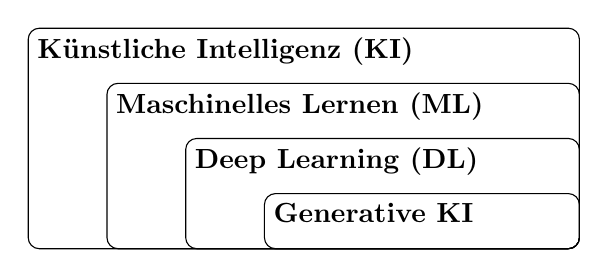
\begin{tikzpicture}
            \node[rectangle, draw, rounded corners, minimum height=2.8cm, minimum width=7cm] (ai) {};

            \node[rectangle, draw, rounded corners, minimum height=2.1cm, minimum width=6cm, anchor=south east] (ml) at (ai.south east) {};

            \node[rectangle, draw, rounded corners, minimum height=1.4cm, minimum width=5cm, anchor=south east] (dl) at (ml.south east) {};

            \node[rectangle, draw, rounded corners, minimum height=0.7cm, minimum width=4cm, anchor=south east] (genai) at (dl.south east) {};

            \node[anchor=north west] at (ai.north west) {
                \textbf{Künstliche Intelligenz (KI)}
            };

            \node[anchor=north west] at (ml.north west) {
                \textbf{Maschinelles Lernen (ML)}
            };

            \node[anchor=north west] at (dl.north west) {
                \textbf{Deep Learning (DL)}
            };

            \node[anchor=north west] at (genai.north west) {
                \textbf{Generative KI}
            };
        \end{tikzpicture}
    }
    \caption{Begriffe im Rahmen von künstlicher Intelligenz.}
    \label{sec1:intro:fig:ai-terms}
\end{figure}
\noindent
Künstliche Intelligenz ist ein Überbegriff und bezeichnet den Ansatz, mit Maschinen intelligentes menschliches Verhalten nachzuahmen, um dadurch Probleme zu lösen \cite{ai-ml-dl}.
Maschinelles Lernen ist ein Überbegriff für die Technologien, die eingesetzt werden, um künstliche Intelligenz zu erreichen \cite{ai-ml-dl}.
Deep Learning ist eine Weiterentwicklung des maschinellen Lernens und macht Gebrauch von neuronalen Netzwerken, welche dem menschlichen Gehirn nachempfunden sind \cite{ai-ml-dl}.
Generative KI ist ein besonderer Bereich der künstlichen Intelligenz und ein Sammelbegriff für auf künstlicher Intelligenz basierender Systeme, mit welcher neue und originelle Inhalte erstellt werden können \cite{gen-ai-definition}.

Die enormen und komplexen Datenmengen, die mittlerweile im Internet generiert werden \cite{global-mobile-data-usage}, verstärken das Potenzial von maschinellem Lernen, sowie aber auch ihre Notwendigkeit \cite{mckinsey-generative-ai}.
Noch bis vor Kurzem war maschinelles Lernen auf vorausschauende Modelle beschränkt, die nur in der Lage waren, Beobachtungen vorzunehmen und Muster zu erkennen.
Durch generative künstliche Intelligenz, wie ChatGPT-3.5 \cite{chatgpt} oder Dall-E 2 \cite{dall-e-2}, konnte ein Durchbruch erzielt werden, welcher ermöglicht, neue Inhalte zu erzeugen \cite{mckinsey-generative-ai}.

In dieser Arbeit wird untersucht, ob und inwiefern generative KI verwendet werden kann, um die semantische Lücke zu schließen und inwieweit generative KI geeignet ist, präzise Erklärungen bzw. geeignete semantische Darstellungen aus identifizierten Merkmalen zu generieren.


%% Motivation
\subsection{Motivation}
\label{sec1:intro:subsec:motivation}
Bei dieser Arbeit handelt es sich um eine Bachelorarbeit im Forschungsumfeld von Prof. Dr.-Ing. Stefan Wagenpfeil am Lehrgebiet Multimedia und Internetanwendungen (MMIA) von Prof. Dr.-Ing. Matthias Hemmje.
Schon vor der Bachelorarbeit bin ich über das von diesem Lehrgebiet angebotene Fachpraktikum Multimedia Information Retrieval mit dem Bereich \mmir{} in Kontakt gekommen.
Da mich das Fachpraktikum und das Themengebiet des \mmir{} sehr interessiert und begeistert hat, schreibe ich nun in diesem Lehrgebiet meine Bachelorarbeit, um meine Fähigkeiten auszubauen und mein Wissen zu vertiefen.

Das Lehrgebiet MMIA hat zum Zwecke der Forschung im Bereich des \mmir{} das Forschungsprojekt \gmafi{} ins Leben gerufen.
Dieses Forschungsprojekt wurde entwickelt, um aktuelle Missstände und Probleme des einfachen \mmir{} auf intelligente Art und Weise zu adressieren.
Das \gmaf{} hat dabei zum Ziel, durch eine intelligente Erweiterung von \mmir{} semantische, erklärbare, für Menschen verständliche, effektive, effiziente, kompatible und integrierte Lösungen anzubieten \cite[S.~20]{swa_diss}.
Diese Erweiterung wird \smmiri{} genannt.
\smmir{} führt eine Reihe von Konzepten ein, die über klassisches \mmir{} hinaus gehen.
Hierzu gehören erweiterte Metriken für die Berechnung von Ähnlichkeit oder Empfehlungen, Möglichkeiten der Merkmalsintegration und -fusion, sowie die Erklärbarkeit von Prozessen des \mmir{} und deren Inhalte.
Unter Erklärbarkeit versteht man in diesem Zusammenhang für Menschen verständliche Antworten auf Fragestellungen, wie z.B. die Frage \enquote{Was ist die wichtigste Eigenschaft des Elements?} oder \enquote{Was ist der Unterschied zwischen diesen zwei Bildern?}.
Sollen Antworten auf diese Fragen auf für Menschen verständliche Art und Weise ausgedrückt werden, so müssen diese Antworten auf natürlicher Sprache aufbauen, oder prägnant visuell dargestellt werden.
Ein Beispiel für eine generierte textuelle Erklärung, die auf natürlicher Sprache aufbaut, ist in \cref{sec1:intro:subsec:motivation:fig:gmaf-explain-ui-dog-man-example} zu sehen.
\begin{figure}[!htb]
    \begin{minipage}{0.45\textwidth}
        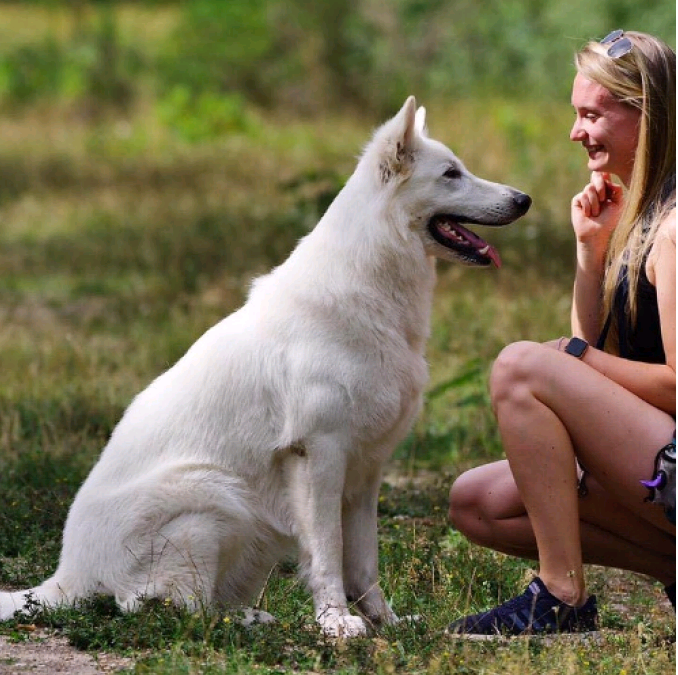
\includegraphics[width=0.769\textwidth]{resources/images/dog_woman.png}
    \end{minipage}%
    \fbox{
            \begin{minipage}{.45\textwidth}
                The picture shows two primary objects.
                  The first object is a dog, the second object is a woman.
                  The dog is white and has black eyes.
                  The woman is smiling and has blonde hair.
                  The woman is wearing shoes, shorts, a top, and a watch.
                  The shoes are blue.
                  The shorts are blue.
                  The top is black.
                  The watch is an Apple Watch.
                  In the background there is grass.
            \end{minipage}
    }
    \caption[Beispiel für eine generierte Erklärung]{Beispiel für eine generierte textuelle Beschreibung eines Bildes im GMAF.}
    \label{sec1:intro:subsec:motivation:fig:gmaf-explain-ui-dog-man-example}
\end{figure}
%\noindent
%\newline
Das \gmaf{} bietet hierfür ein umfangreiches Konzept zur Generierung von textuellen Beschreibungen von \mmir{}-Inhalten in für Menschen lesbarer und verständlicher Form.
Es ist allerdings wichtig anzumerken, dass dieses Konzept statistisch und rein mathematische Ansätze zur Generierung von natürlicher Sprache verfolgt, ohne dabei Methoden maschinellen Lernens zu verwenden.
Diese Ansätze generieren jedoch nur textuelle Beschreibungen auf eine statische Art und Weise.
Zudem können mit diesen Ansätzen keine anderen Formen, wie z.B visuelle Beschreibungen, außer Text generiert werden.
Es ist also erstrebenswert nach einer Lösung zu suchen, mit welcher man sich von diesen statischen Ansätzen lösen kann.
Ein anderer Ansatz, der in den letzten Monaten stark an Popularität gewonnen hat, ist die generative KI.
Generative KI scheint eine vielversprechende Alternative zu einem statischen, statistischen und rein mathematischen Ansatz zu sein.
\newline
Ließen sich mittels generativer KI tatsächlich \mmir{}-Prozesse erklären, so kann dies einen echten Mehrwert für Benutzer darstellen, da diese von präzisen Erklärungen oder visuellen Darstellungen profitieren würden.
Beispiele für Mehrwert für Benutzer können sein:
\begin{itemize}
    \item \textbf{Zeitersparnis.} Generative KI könnte anhand identifizierter Merkmale Datei(en) zusammenfassen und in kürzester Zeit präzise Beschreibungen der Datei(en) erstellen.
    Ein Benutzer müsste für diese Arbeit erheblich mehr Zeit aufwenden.
    \item \textbf{Überblick / Ordnung.} Generative KI könnte anhand identifizierter Merkmale in einer großen Kollektion an Dateien Zusammenhänge erkennen und dem Benutzer eine Beschreibung dieser Zusammenhänge bieten.
    Zusammenhänge können in diesem Fall Muster oder eine für den Benutzer versteckte bzw. nicht ersichtliche Ordnung innerhalb der Dateien sein.
    \item \textbf{Barrierefreiheit.} Es gibt bereits Programme, wie z.B. Screen Readers, die blinden Personen Beschreibungen von Bildern vorlesen.
    Nachteil ist, dass diese Programme abhängig von den im Bild eingebetteten Beschreibungen sind, und viele Bilder im Internet über keine eingebetteten Beschreibungen verfügen.
    Zusätzlich sind diese Beschreibungen meistens von Menschen verfasst \cite{google-ai-accessability}.
    \newline
    Generative KI könnte anhand identifizierter Merkmale Beschreibungen solcher Bilder generieren.
    Diese Beschreibungen könnten in weiteren Schritten von anderen Programmen, oder selbst wieder generativer KI verwendet werden, um diese vorzulesen.
    Auf diese Weise könnte echte Barrierefreiheit erreicht werden.
\end{itemize}

\FloatBarrier

%% Problembeschreibung
\subsection{Problembeschreibung}
\label{sec1:intro:subsec:problems}
Das \gmaf{} bietet bereits ein umfangreiches Konzept zur Erklärbarkeit von Prozessen des \mmir{}.
Die Ansätze, die in diesem Konzept verfolgt werden, sind statisch, in ihrer Anwendung begrenzt und ihre Erklärbarkeit vergleichsweise rudimentär.
In diesem Abschnitt werden diese Probleme angesprochen, umrissen und subsequent Problembeschreibungen definiert.

\subsubsection{Probleme in Bezug auf die Erklärbarkeit}
\label{sec1:intro:subsec:problems:pb:explain}
Das \gmaf{} bietet bereits Verfahren zur Erklärbarkeit von \mmir{}-Prozessen.
Die Ansätze, die mit diesen Verfahren umgesetzt werden, sind allerdings sehr statisch und basieren wiederum auf statistischen und rein mathematischen Ansätzen.
Noch dazu bieten diese Verfahren nur die Erklärbarkeit von \mmir{}-Prozessen anhand von Text.
Es ist allerdings wichtig anzumerken, dass Text nicht die einzige Form der Erklärbarkeit ist.
Eine andere Form der Erklärbarkeit kann mittels Bilder erzielt werden.
So lautet ein bekanntes Sprichwort: \enquote{\textit{Ein Bild sagt mehr als 1000 Worte}}.
Dieses Sprichwort will zum Ausdruck bringen, dass Bilder, im Vergleich zu Text, ebenfalls komplexe Sachverhalte und Wissen prägnant und in für Menschen verständlicher Form zum Ausdruck bringen können.
Ein Beispiel hierfür wäre eine Bauanleitung zu einem Lego-Set.
Ein Beispiel für eine Bauanleitung zum Bauen eines Osterkükens ist in \cref{sec1:intro:subsec:problems:fig:lego-instructions} zu sehen.
Die Bauanleitung veranschaulicht dabei die einzelnen Aufbauschritte durch fortwährende Nummerierung und Abbildungen.
\begin{figure}[!htb]
    \centering
    \copyrightbox[b]{
            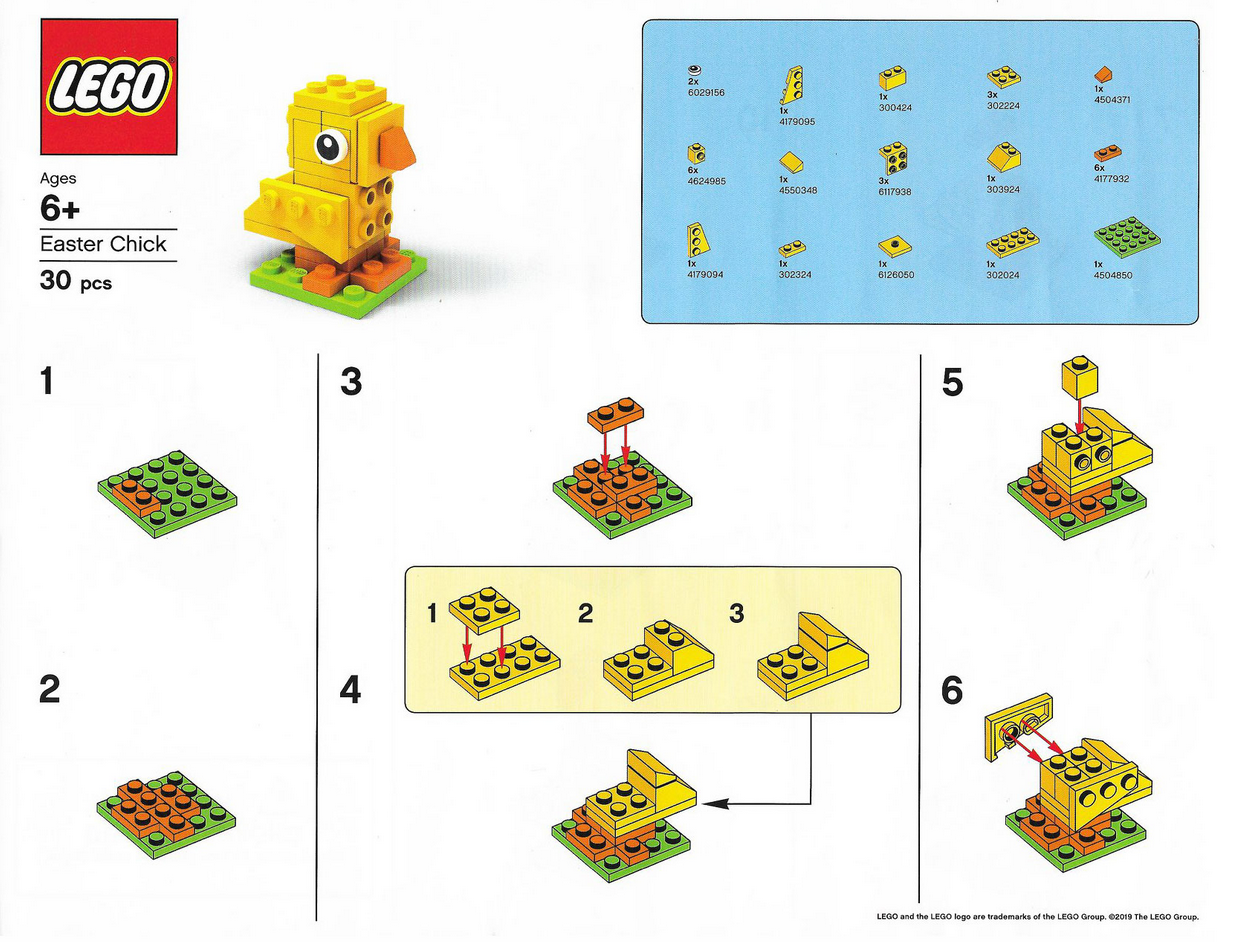
\includegraphics[width=0.8\linewidth]{resources/images/lego-instructions.png}
        }
        {%
        \textcolor{black}{%
            %Haftungsausschluss: \copyright{} 2023 Lego Gruppe - Diese Arbeit ist unabhängig und wurde von der LEGO Gruppe weder genehmigt noch gesponsert.
            Haftungsausschluss: LEGO \textsuperscript{\textregistered{}} und das LEGO Logo sind Marken der LEGO Unternehmensgruppe. 
            \newline
            \copyright{} 2023 Lego Gruppe. Diese Arbeit ist unabhängig und wurde von der LEGO Gruppe weder genehmigt, noch gesponsort.
        }
    }
    \caption{Bauanleitung für ein Lego-Set \cite{lego-easter-chick}.}
    \label{sec1:intro:subsec:problems:fig:lego-instructions}
\end{figure}

Ein konkretes Anwendungsbeispiel für die Erklärbarkeit in Form von Bildern wäre im Rahmen des \mmir{} die Generierung von Vorschaubildern für eine Textdatei.
\cref{sec1:intro:subsec:problems:fig:mmir-example-1} zeigt ein Beispiel für ein von Dall-E 2 \cite{dall-e-2} generiertes Vorschaubild für ein Gedicht über einen Schmetterling \cite{butterfly-poem}.
Anhand der in der Textdatei identifizierten Merkmale könnte eine generative KI, wie z.B Dall-E 2, ein Vorschaubild generieren, um somit den Inhalt des Textes visuell zu erklären.
\begin{figure}[!htb]
    \centering
    \resizebox{\textwidth}{!}{
        \begin{tikzpicture}
            \def\corner{5mm};
             \def\cornerradius{0.2mm};
             \def\lwidth{0.3mm};
             \def\h{3.5cm};
             \def\w{4.8cm};
             \def\nline{10};
             \def\iconmargin{1mm};
             \def\topmargin{2mm};
             \foreach[count=\i] \filename in {\textbf{Schmetterling}}
             {
               \coordinate (nw) at ($(0,0)$);
               \coordinate (ne0) at ($(nw) + (\w, 0)$);
               \coordinate (ne1) at ($(ne0) - (\corner, 0)$);
               \coordinate (ne2) at ($(ne0) - (0, \corner)$);
               \coordinate (se) at ($(ne0) + (0, -\h)$);
               \filldraw [-, line width = \lwidth, fill=white] (nw) -- (ne1) -- (ne2)
                [rounded corners=\cornerradius]--(se) -- (nw|-se) -- cycle;
               \draw [-, line width = \lwidth] (ne1) [rounded corners=\cornerradius]-- (ne1|-ne2) -- (ne2);
               \node [anchor=north west] at (nw) {\fontsize{10}{7}\selectfont \filename};
               \node [anchor=north west, text width=4.8cm] (poem) at ([yshift=-0.6cm]nw) {%
                  \begin{varwidth}{4.8cm}
                      \fontsize{6}{7.2}\selectfont
                      Fliege kleiner Schmetterling \newline
                      mach dir die Welt zu Eigen \newline
                      du kannst mit deiner Leichtigkeit \newline
                      uns noch so vieles zeigen \newline
                      zum Beispiel, dass es weiter geht \newline
                      auch wenn man lang im Dunkel steht \newline
                      am Lebensanfang nur gekrochen \newline
                      hast du die Freiheit nun gerochen \newline
                      du zeigst den Wandel uns im Leben \newline
                      so ist das Leben, Wandel eben. \newline
                      \vspace{\fill}
                  \end{varwidth}
               };
             }

             \draw[-latex, line width=0.7mm] (5.1, -1.7) -- node[above] {Dall-E 2} (7.5, -1.7);

             \node[] (img) at (10, -1.75) {
                \includegraphics[width=4.5cm]{resources/images/DALL·E 2023-04-19.png}
             };

             %\draw[-latex, line width=0.7mm] ([xshift=5mm]poem.east) -- node[above] {Dall-E 2} ([xshift=-5mm]img.west);

        \end{tikzpicture}
    }
    \caption[Beispiel für ein generiertes Vorschaubild]{Ein von Dall-E 2 generiertes Vorschaubild.}
    \label{sec1:intro:subsec:problems:fig:mmir-example-1}
\end{figure}

Ein Vorschaubild kann sich dann als sinnvoll erweisen, wenn viele Dateien zu verwalten sind und Benutzer nicht die Zeit haben diese einzeln zu durchforsten.
Durch einen kurzen Blick auf das Vorschaubild könnte ein Benutzer die Datei einordnen und sich besser zurechtfinden.

Ein weiteres Anwendungsbeispiel wäre die Gemeinsamkeit/Differenz aus einer Kollektion an Bildern.
Die als Gemeinsamkeit/Differenz identifizierten Merkmale könnten in diesem Beispiel ebenfalls konkret mittels eines Bildes kurz und prägnant visuell dargestellt werden.
Diese Art der visuellen Erklärung kann sich dann als sinnvoll erweisen, wenn viele Bilder auf ihre Merkmale hin untersucht werden sollen.
Ein Benutzer kann hier schnell den Überblick verlieren.

Statistische und rein mathematische Ansätze reichen für diese Beispiele nicht mehr aus.
Ein anderer, vielversprechender Ansatz, um die Erklärbarkeit von Prozessen des \mmir{} zu erreichen, liegt in generativer KI. Mittels generativer KI könnten anhand identifizierter Merkmale eigenständig neuartige Multimedia-Inhalte, wie Texte oder Bilder, erzeugt werden, die zur Erklärbarkeit von \mmir{}-Prozessen dienen könnten.

Je nach Anwendungsbereich variieren die Anforderungen an Erklärungen allerdings erheblich.
Somit ist ein weiterer wichtiger Aspekt die Anpassungsmöglichkeiten von Erklärungen in Abhängigkeit ihrer Anwendungsfälle.
%So wird \smmir{} für die Erkennung sicherheitsrelevanter Zustände im Bereich Automotive eingesetzt.
%Hier werden kurze, präzise Erklärungen benötigt.
%Im Gegensatz dazu steht der Bereich des Wissensmanagements, in welchem \smmir{} ebenfalls Anwendung für Fragestellungen findet.
%In diesem Bereich werden ausführliche Erklärungen benötigt.
So wird \smmir{} für die Erkennung sicherheitsrelevanter Zustände im Bereich der Automobilindustrie, auch Automotive genannt, eingesetzt \cite{jour-smmir}.
Sicherheitsrelevante Zustände in einem Kraftfahrzeug sind Zustände, die für eine reibungslose Fahrt und Funktion sorgen, oder unterstützend und im Sinne des Autofahrers eingreifen oder im Ernstfall zum Schutz von Insassen und Außenstehenden beitragen \cite{kfz-safety-states}.
Ein Beispiel für eine unterstützende Funktion kann in Form von HeadUp-Displays (HUD) gefunden werden und ist in \cref{sec1:intro:subsec:problems:fig:automotive-hud} zu sehen. Das HeadUp-Dispaly projiziert sicherheitsrelevante Informationen, wie z.B. die Geschwindigkeit auf die Windschutzscheibe.
\begin{figure}[htb]
    \centering
    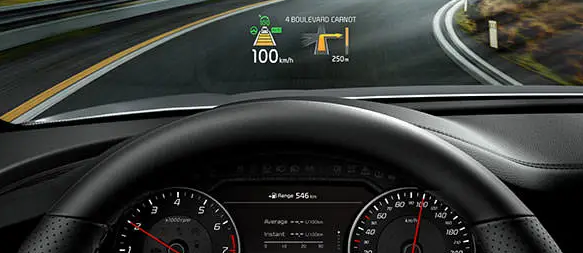
\includegraphics[width=0.9\textwidth]{resources/images/automotive-hud.png}
    \caption{HeadUp-Display in einem Kraftfahrzeug \cite{head-up-display}.}
    \label{sec1:intro:subsec:problems:fig:automotive-hud}
\end{figure}
Da im Bereich Automotive schnelle Entscheidungen getroffen werden müssen, werden hier kurze, präzise Erklärungen benötigt.
Es ist also in Bezug auf die Erklärbarkeit notwendig Eigenschaften, wie z.B. die Länge der Erklärung, anpassen zu können.
Das \gmaf{} bietet bereits eine Benutzungsschnittstelle, die es ermöglicht Anpassungen von textuellen Erklärungen vorzunehmen. Diese Benutzungsschnittstelle ist in \cref{sec1:intro:subsec:problems:fig:explain-ui} zu sehen und zeigt die Elemente, die zur Anpassung von textuellen Erklärungen vorgesehen sind.
\begin{figure}[htb]
    \centering
    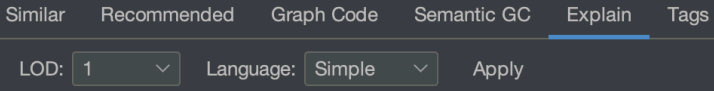
\includegraphics[width=0.7\textwidth]{resources/images/explain-ui.png}
    \caption{Benutzungsschnittstelle im \gmaf{} zum Anpassen von Erklärungen.}
    \label{sec1:intro:subsec:problems:fig:explain-ui}
\end{figure}
Diese Benutzungsschnittstelle bietet allerdings nur grobe Möglichkeiten zur Anpassung von textuellen Erlärungen, wie die Anpassung der Komplexität der textuellen Beschreibung.
Möglichkeiten zur Anpassung der Länge der textuellen Beschreibungen ermöglicht diese Schnittstelle zum Beispiel jedoch nicht. Schlussendlich kann in Bezug auf die Erklärbarkeit von \mmir{}-Prozessen folgende Problembeschreibung formuliert werden:

\problemstmt{} Generative KI ist aktuell nicht für die Erklärbarkeit von \mmir{}-Prozessen nutzbar.

\subsubsection{Probleme in Bezug auf die Integration}
\label{sec1:intro:subsec:problems:pb:integration}
Damit generative KI-Systeme aus identifizierten Merkmalen präzise und für Menschen verständliche Erklärungen generieren können, müssen die identifizierten Merkmale als Eingabedaten in die jeweiligen Systeme überführt werden.
Das \gmaf{} bietet keine Möglichkeiten zur Anbindung von Systemen, die generative KI anbieten, sowie kein Modell zur Übersetzung von identifizierten Merkmalen in Eingabedaten für entsprechende Systeme.
Folglich gibt es auch keine Modellierung, die die Anpassung der Eingabedaten ermöglicht, um die in \cref{sec1:intro:subsec:problems:pb:explain} benannten Modifikationen von Erklärungen zu ermöglichen.
Gelingt eine Integration von generativen KI-Systemen, so kann dies einen echten Mehrwert für Benutzer darstellen, sofern dadurch verbesserte und originellere Erklärungen von \mmir{}-Prozessen generiert werden.
Besonders die Möglichkeit, je nach Anforderung die Eingabedaten anzupassen, kann für Benutzer von Nutzen sein.
Schlussendlich kann in Bezug auf die Integration folgende Problembeschreibung formuliert werden:

\problemstmt{} Das \gmaf{} bietet keine Integration generativer KI.

\subsubsection{Allgemeine Zielsetzung}
\label{sec1:intro:subsec:objective}
Aus den in \cref{sec1:intro:subsec:problems:pb:explain} und \cref{sec1:intro:subsec:problems:pb:integration} beschriebenen Problembereichen lassen sich zwei direkte Probleme erfassen:
Die im \gmaf{} implementierten Konzepte zur Erklärung von \mmir{}-Prozessen sind noch sehr statisch und bieten nur Erklärungen in Form von Text, sowie die Integration besserer Lösungen zur Erklärbarkeit von \mmir{}-Prozessen.
Die Motivation dieser Arbeit besteht darin, dass die bereits implementierten Konzepte im \gmaf{} in Bezug auf die Erklärbarkeit von \mmir{}-Prozessen noch großen Raum für Verbesserung aufweisen.
Verbesserung wird sich durch das Anbinden von generativer KI versprochen, da generative KI in der Lage zu sein scheint auf kreative Weise neuartige Inhalte zu generieren.

Werden nun die Problembeschreibungen zusammengefasst, so wird das übergeordnete Ziel sichtbar:

\textit{Die im \gmaf{} implementierten Konzepte zur Erklärung von \mmir{}-Prozessen sollen durch \textbf{generative KI} abgelöst werden, um \textbf{bessere Erklärungen}, sowie \textbf{andere Formen von Erklärungen} zu ermöglichen.}

\clearpage
Anhand der in diesem Abschnitt beschriebenen Problembeschreibungen und des allgemeinen Ziels können nun im nächsten \cref{sec1:intro:subsec:research-questions} folgende Forschungsfragen formuliert werden. Im darauffolgenden \cref{sec1:intro:subsec:methodology-goals} wird genauer auf die Methodik dieser Arbeit, sowie die konkreteren Ziele eingegangen.

\subsection{Forschungsfragen}
\label{sec1:intro:subsec:research-questions}
Um die im vorigen Abschnitt definierten Problembeschreibungen zu adressieren, werden folgende Forschungsfragen definiert:
\begin{itemize}
    \item \researchquestion{} Kann generative KI für die Erklärbarkeit von \mmir{}-Prozessen genutzt werden?
    \item \researchquestion{} Wie lässt sich generative KI in das \gmaf{} integrieren?
\end{itemize}

\subsection{Methodik und Ziele}
\label{sec1:intro:subsec:methodology-goals}
Um die in \cref{sec1:intro:subsec:problems} identifizierten Probleme und subsequent die im vorigen \cref{sec1:intro:subsec:research-questions} formulierten Forschungsfragen strukturiert beantworten zu können, wird diese Arbeit auf der vielfach bewährten Methodik von Nunamaker \cite{nunamaker} aufbauen.
Die Methodik nach Nunamaker teilt ein zu lösendes Problem anhand von Recherche und Entwicklung in vier Phasen der Problemlösung auf.
\newline
Diese vier Phasen lauten:
\begin{enumerate}
    \setlength{\itemsep}{0pt}
    \item Beobachtungsphase
    \item Theoriebildungsphase
    \item Systementwicklungs - bzw. Implementierungsphase
    \item Experimentphase
\end{enumerate}
\begin{figure}[htb]
    \centering
    \resizebox*{0.75\textwidth}{!}{
        \begin{minipage}{\textwidth}
            \begin{tcolorbox}[
                enhanced, width=\textwidth, height=\textwidth, colback=white, colframe=black,
                overlay={
                    \tikzset{
                        exstyle/.style={-{Triangle[angle=90:6pt,length=3mm,fill=black]}}
                    }
                    \def\rad{\textwidth-2.5cm}
                    \node [circle, minimum size=\rad] (c) at ([yshift=-0.8cm]frame.center) {};
                    \def\labellist{
                          \shortstack{
                            \Large \textbf{Beobachtung} \\
                            \rule{3cm}{1pt} \\
                            \footnotesize
                            Umfragestudien, \\ 
                            \footnotesize
                            Fallstudien, \\
                            \footnotesize
                            Feldforschung
                          }, 
                          \shortstack{
                            \Large \textbf{Experiment} \\
                            \rule{3cm}{1pt} \\
                            \footnotesize
                            Computersimulationen,\\ 
                            \footnotesize
                            Feldexperimente, \\
                            \footnotesize
                            Laborexperimente
                          },
                          \shortstack{
                            \Large \textbf{Theorie} \\ \Large \textbf{Bildung} \\
                            \rule{3cm}{1pt} \\
                            \footnotesize
                            konzept. Rahmen-\\ 
                            \footnotesize
                            bedingungen, mathe\\
                            \footnotesize
                            matische Modelle\\
                            \footnotesize 
                            Methoden
                          }
                    }
                    
                    \foreach [count=\i] \x in \labellist {
                        
                        \node (n\i) [draw, fill=white, minimum size=0cm, inner sep=0mm, circle] at (c.\i*360/3+90) {
                            \scalebox{0.8}{
                                \x
                            }
                        };
                    }
                    \node (nm) [draw, fill=white, minimum size=0cm, inner sep=0mm, circle] at (c.center) {
                        \scalebox{0.8}{
                            \shortstack{
                                \Large \textbf{System} \\ \Large \textbf{Entwicklung} \\
                                \rule{3cm}{1pt} \\
                                \footnotesize
                                Produktentwicklung,\\ 
                                \footnotesize
                                Technologietransfer, \\
                                \footnotesize
                                Prototyping
                            }
                        }
                    };
                    \node [anchor=south east, rectangle, minimum width=4cm, rounded corners, text=white, fill=black, inner sep=1.7mm] at (frame.south east) {
                        \textbf{nach J. Nunamaker}
                    };

                    \draw[exstyle] (nm.200) -- (n1.40);
                    \draw[exstyle] (n1.25) -- (nm.215);

                    \draw[exstyle] (nm.340) -- (n2.140);
                    \draw[exstyle] (n2.155) -- (nm.325);

                    \draw[exstyle] (nm.{83}) -- (n3.{277});
                    \draw[exstyle] (n3.{263}) -- (nm.{97});

                    \draw[exstyle, bend left=41.5](n3.0) to (n2.60);
                    \draw[exstyle, bend left=41.5](n2.240) to (n1.300);
                    \draw[exstyle, bend left=41.5](n1.120) to (n3.180);

                    \draw[exstyle, bend right=41.5](n2.78) to (n3.342);
                    \draw[exstyle, bend right=41.5](n1.318) to (n2.222);
                    \draw[exstyle, bend right=41.5](n3.198) to (n1.102);

                    \node[circle, fill=white, draw, minimum size=1cm] at (n1.71) {1};
                    \node[circle, fill=white, draw, minimum size=1cm] at (n3.25) {2};
                    \node[circle, fill=white, draw, minimum size=1cm] at (nm.45) {3};
                    \node[circle, fill=white, draw, minimum size=1cm] at (n2.110) {4};
                }
            ]
            \end{tcolorbox}
        \end{minipage}
    }
    \caption{Phasen der Problemlösung nach Nunamaker \cite{nunamaker}.}
    \label{sec1:intro:subsec:methodology-goals:fig:nunamaker}
\end{figure}
In der Beobachtungsphase werden im Rahmen einer Recherche Informationen gesammelt.
In der Theoriebildungsphase werden Konzepte für Lösungen konzipiert und modelliert.
Die Systementwicklungs bzw. Implementierungsphase beschäftigt sich mit der Entwicklung von Lösungen, basierend auf den Theorien aus der Theoriebildungsphase bzw. Beobachtungen aus der Beobachtungsphase, und welche in der letzten Phase, der Experimentphase evaluiert werden können.
Diese Phasen sind eng miteinander verwoben, und jede Phase mündet mit seinem Ergebnis in den anderen Phasen und trägt zu diesen bei.
Durch die Methodik von Nunamaker wird sichergestellt, dass jedes Forschungsziel eindeutig einer Problembeschreibung zugeordnet werden kann.

Die Anwendung der Methodik nach Nunamaker führt für jede Forschungsfrage zu jeweils vier Forschungszielen, die in jeweils einem Unterkapitel behandelt werden.
Dies führt insgesamt zu acht Forschungsaufgaben, die mit dieser Arbeit behandelt werden.
Die anfängliche Planung der Forschungsziele ist in \cref{sec1:intro:table:research-questions} einsehbar.
Die Benennung der Forschungsaufgaben folgt einem einheitlichen Schema und ergibt sich aus dem Namen des jeweiligen Forschungsziels, erweitert durch einen Buchstaben als Anhängsel, z.B. \enquote{O}
 für \textit{Observation}/Beobachtung, \enquote{TB} für \textit{Theory Building}/Theoriebildung, \enquote{I} für \textit{Implementation}/Implementierung und \enquote{E} für \textit{Experiment}.
 \clearpage
{
    \def\arraystretch{1.1}%
    \begin{xltabular}{\linewidth}{
            @{}
            >{
                \hsize=0.15\linewidth
                \raggedright\arraybackslash
            }X
            >{
                \hsize=0.75\linewidth
                \raggedright\arraybackslash
            }X
            >{
                \hsize=0.1\linewidth
                \centering\arraybackslash
            }X
            @{}
    }

    % First Header

    \caption{Aufschlüsselung der Forschungsfragen auf Forschungsziele} 
    \label{sec1:intro:table:research-questions} \\
        
    \toprule
    \multicolumn{3}{
        >{
            \hsize=\linewidth\centering\arraybackslash
        }X
    }
    {
        \textbf{Forschungsfragen}
    } \\ 
    \midrule
         
    \textbf{FZ} & \multicolumn{1}{c}{\textbf{Beschreibung}} & \textbf{PB} \\ 
    \midrule
    
    \endfirsthead

    % Normal Head

    \toprule
    \multicolumn{3}{
        >{
            \hsize=\linewidth\centering\arraybackslash
        }X
    }
    {
        \textbf{Forschungsfragen}
    } \\ 
    \midrule
         
    \textbf{FZ} & \multicolumn{1}{c}{\textbf{Beschreibung}} & \textbf{PB} \\ 
    \midrule
    
    \endhead
        
    % Lower Rows

    \multicolumn{3}{
        >{
            \hsize=\linewidth\centering\arraybackslash
        }X
    }
    {
        \textbf{Erklärbarkeit von MMIR mittels generativer KI}
    } \\ \midrule

    FZ 1.1/O 
    & 
    Recherche zur Erklärbarkeit von MMIR mittels generativer KI
    & PB1 \\

    \midrule

    FZ 1.2/TB 
    & 
    Modellierung zur Erklärbarkeit von MMIR mittels generativer KI
    & PB1 \\

    \midrule

    FZ 1.3/I
    & 
    Implementierung zur Erklärbarkeit von MMIR mittels generativer KI
    & PB1 \\

    \midrule

    FZ 1.4/E 
    & 
    Experiment zur Erklärbarkeit von MMIR mittels generativer KI
    & PB1 \\

    \midrule

    \multicolumn{3}{
        >{
            \hsize=\linewidth\centering\arraybackslash
        }X
    }
    {
        \textbf{Integration generativer KI in das GMAF}
    } \\ \midrule

    FZ 2.1/O 
    & 
    Recherche zur Integration generativer KI in das GMAF
    & PB2 \\

    \midrule

    FZ 2.2/TB 
    & 
    Modellierung zur Integration generativer KI in das GMAF
    & PB2 \\

    \midrule

    FZ 2.3/I
    & 
    Implementierung zur Integration generativer KI in das GMAF
    & PB2 \\

    \midrule

    FZ 2.4/E 
    & 
    Experiment zur Integration generativer KI in das GMAF
    & PB2 \\
        
    \bottomrule 

    \end{xltabular}
}
\noindent
Um sicherzustellen, dass alle Forschungsziele durch den Inhalt dieser Arbeit abgedeckt werden, entspricht die Struktur dieses Dokuments direkt dem Ansatz nach Nunamaker.
Der Ansatz und Aufbau der Arbeit wird im nächsten Abschnitt behandelt.

\subsection{Ansatz und Aufbau der Arbeit}
\label{sec1:intro:subsec:approach-structure}
Die Struktur dieser Arbeit ergibt sich 1:1 aus der Methodik von Nunamaker \cite{nunamaker} und folgt seiner Modellierung.
Ein Überblick auf die Struktur dieser Arbeit und Nunamakers Ansatz ist in \cref{sec1:intro:subsec:approach-structure:fig:outline-nunamaker}.
Die entsprechenden Forschungsziele werden, je nach Phase der Modellierung nach Nunamaker, umgeordnet und in die jeweiligen Kapitel dieser Arbeit umgruppiert.
\clearpage
\begin{figure}[htb]
    \centering
    \newlength{\w}
    \setlength{\w}{0.9\textwidth}
    \resizebox*{\w}{!}{
        \begin{tikzpicture}

            \tikzset{
                exstyle/.style={-{Triangle[angle=90:6pt,length=3mm,fill=black]}},
                pbstyle/.style={-{Triangle[angle=90:3pt,length=1.5mm,fill=black]}}
            }

            \node[rectangle, minimum width=\w, minimum height=\w-2cm] (outline) {};

            \newlength{\nuna}
            \setlength{\nuna}{0.6\w}

            \node[anchor=south east, draw, rectangle, rounded corners, minimum width=\nuna, minimum height=\nuna] (nuna) at (outline.south east) {};

            \node [anchor=south east, draw, rectangle, rounded corners, text=white, fill=black] at (nuna.south east) {
                \scalebox{0.5}{
                    \textbf{nach J. Nunamaker}   
                }
            };

            \node[rectangle, rounded corners, minimum width=\nuna, minimum height=\nuna, inner sep=0mm] at ([yshift=-0.1cm]nuna.center) {
                \resizebox*{\nuna}{\nuna}{
                    \begin{tikzpicture}[transform shape]

                        \newlength{\radius}
                        \setlength{\radius}{\textwidth-2.5cm}
                        \node[circle, minimum size=\radius] (c) at (nuna.center) {};

                        \def\labellist{
                            \shortstack{
                                \Large \textbf{Beobachtung} \\
                                \rule{3cm}{1pt} \\
                                \footnotesize
                                Umfragestudien, \\ 
                                \footnotesize
                                Fallstudien, \\
                                \footnotesize
                                Feldforschung
                            }, 
                            \shortstack{
                                \Large \textbf{Experiment} \\
                                \rule{3cm}{1pt} \\
                                \footnotesize
                                Computersimulationen,\\ 
                                \footnotesize
                                Feldexperimente, \\
                                \footnotesize
                                Laborexperimente
                            },
                            \shortstack{
                                \Large \textbf{Theorie} \\ \Large \textbf{Bildung} \\
                                \rule{3cm}{1pt} \\
                                \footnotesize
                                konzept. Rahmen-\\ 
                                \footnotesize
                                bedingungen, mathe\\
                                \footnotesize
                                matische Modelle\\
                                \footnotesize 
                                Methoden
                            }
                        }

                        \foreach [count=\i] \x in \labellist {
                            \node (n\i) [draw, fill=white, minimum size=0cm, inner sep=0mm, circle] at (c.\i*360/3+90) {
                                \scalebox{0.8}{
                                    \x
                                }
                            };
                        }
                        \node (nm) [draw, fill=white, minimum size=0cm, inner sep=0mm, circle] at (c.center) {
                            \scalebox{0.8}{
                                \shortstack{
                                    \Large \textbf{System} \\ \Large \textbf{Entwicklung} \\
                                    \rule{3cm}{1pt} \\
                                    \footnotesize
                                    Produktentwicklung,\\ 
                                    \footnotesize
                                    Technologietransfer, \\
                                    \footnotesize
                                    Prototyping
                                }
                            }
                        };

                        \draw[exstyle] (nm.200) -- (n1.40);
                        \draw[exstyle] (n1.25) -- (nm.215);
    
                        \draw[exstyle] (nm.340) -- (n2.140);
                        \draw[exstyle] (n2.155) -- (nm.325);
    
                        \draw[exstyle] (nm.{83}) -- (n3.{277});
                        \draw[exstyle] (n3.{263}) -- (nm.{97});
    
                        \draw[exstyle, bend left=41.5](n3.0) to (n2.60);
                        \draw[exstyle, bend left=41.5](n2.240) to (n1.300);
                        \draw[exstyle, bend left=41.5](n1.120) to (n3.180);
    
                        \draw[exstyle, bend right=41.5](n2.78) to (n3.342);
                        \draw[exstyle, bend right=41.5](n1.318) to (n2.222);
                        \draw[exstyle, bend right=41.5](n3.198) to (n1.102);
                        
                    \end{tikzpicture}
                }
            };

            %\node[draw, rectangle, rounded corners, fill=gray!10] at ([xshift=1.9cm, yshift=1cm]n1.340) {
            %    \tiny Kapitel 2
            %};

            \newlength{\struc}
            \setlength{\struc}{0.47\w}

            \node[anchor=south west, draw, rectangle, rounded corners, minimum width=\struc, minimum height=3.74cm] (struc) at ([yshift=0.4cm]nuna.north west) {};

            \node[anchor=north, minimum width=\struc, draw, rectangle, rounded corners, text=white, fill=black] at (struc.north){
                \scalebox{0.5}{
                    \textbf{Struktur der Arbeit}
                }
            };

            \node[anchor=north west, draw, rectangle, rounded corners, fill=gray!10] (chap1) at ([xshift=0.1cm, yshift=-0.5cm]struc.north west) {
                \tiny Kapitel 1
            };

            \node[anchor=north west, draw, rectangle, rounded corners, fill=gray!10] (chap2) at ([xshift=0.1cm, yshift=-1.04cm]struc.north west) {
                \tiny Kapitel 2
            };

            \node[anchor=north west, draw, rectangle, rounded corners, fill=gray!10] (chap3) at ([xshift=0.1cm, yshift=-1.58cm]struc.north west) {
                \tiny Kapitel 3
            };

            \node[anchor=north west, draw, rectangle, rounded corners, fill=gray!10] (chap4) at ([xshift=0.1cm, yshift=-2.12cm]struc.north west) {
                \tiny Kapitel 4
            };

            \node[anchor=north west, draw, rectangle, rounded corners, fill=gray!10] (chap5) at ([xshift=0.1cm, yshift=-2.66cm]struc.north west) {
                \tiny Kapitel 5
            };

            \node[anchor=north west, draw, rectangle, rounded corners, fill=white] (chap6) at ([xshift=0.1cm, yshift=-3.2cm]struc.north west) {
                \tiny Kapitel 6
            };

            \node[anchor=west] at ([xshift=0.1cm]chap1.east) {
                \tiny Einleitung / Motivation
            };

            \node[anchor=west] at ([xshift=0.1cm]chap2.east) {
                \tiny Stand der Wissenschaft und Technik
            };

            \node[anchor=west] at ([xshift=0.1cm]chap3.east) {
                \tiny Modellierung / Design
            };

            \node[anchor=west] at ([xshift=0.1cm]chap4.east) {
                \tiny Implementierung
            };

            \node[anchor=west] at ([xshift=0.1cm]chap5.east) {
                \tiny Evaluierung
            };

            \node[anchor=west] at ([xshift=0.1cm]chap6.east) {
                \tiny Zusammenfassung / Fazit
            };

            \newlength{\chap}
            \setlength{\chap}{4.2cm}

            \node[anchor=south west, minimum width=\chap, minimum height=8cm, draw, rectangle, rounded corners] (chapter1) at (outline.south west) {};


            
            \node[anchor=center, draw, rectangle, rounded corners, fill=gray!10] (pbn) at ([yshift=-0.8cm]chapter1.north) {
                \tiny PB
            };

            \node[anchor=center, draw, rectangle, rounded corners, fill=gray!10] (pb1n) at ([xshift=-1cm, yshift=-2.8cm]chapter1.north) {
                \tiny PB1
            };

            \node[anchor=center, draw, rectangle, rounded corners, fill=gray!10] (pb2n) at ([xshift=1cm, yshift=-2.8cm]chapter1.north) {
                \tiny PB2
            };

            \node[anchor=center, draw, rectangle, rounded corners, fill=gray!10] (resq1) at ([xshift=-1cm, yshift=-4.5cm]chapter1.north) {
                \tiny FF1
            };

            \node[anchor=center, draw, rectangle, rounded corners, fill=gray!10] (resq2) at ([xshift=1cm, yshift=-4.5cm]chapter1.north) {
                \tiny FF2
            };

            

            \node[anchor=west, draw, rectangle, rounded corners, fill=gray!10] (resto) at ([xshift=-0.4cm, yshift=-5.85cm]chapter1.north) {
                \tiny FZ 1.1/O
            };

            \node[anchor=west, draw, rectangle, rounded corners, fill=gray!10] (resttb) at ([xshift=-0.4cm, yshift=-6.45cm]chapter1.north) {
                \tiny FZ 1.2/TB
            };

            \node[anchor=west, draw, rectangle, rounded corners, fill=gray!10] (resti) at ([xshift=-0.4cm, yshift=-7.05cm]chapter1.north) {
                \tiny FZ 1.3/I
            };

            \node[anchor=west, draw, rectangle, rounded corners, fill=gray!10] (reste) at ([xshift=-0.4cm, yshift=-7.65cm]chapter1.north) {
                \tiny FZ 1.4/E
            };

            \draw[pbstyle, line width=0.3mm] (pbn) -- (pb1n);
            \draw[pbstyle, line width=0.3mm] (pbn) -- (pb2n);

            \draw[pbstyle, line width=0.3mm] (pb1n) -- (resq1);
            \draw[pbstyle, line width=0.3mm] (pb2n) -- (resq2);
            
            \draw[pbstyle, line width=0.3mm] (resq1) |- (reste);
            \draw[pbstyle, line width=0.3mm] (resq1) |- (resti);
            \draw[pbstyle, line width=0.3mm] (resq1) |- (resttb);
            \draw[pbstyle, line width=0.3mm] (resq1) |- (resto);

            

            \node[align=left, anchor=north, minimum width=\chap, draw, rectangle, rounded corners, text=white, fill=black, text width=0.9\chap] (pb) at (chapter1.north){
                \tiny \textbf{Problem}
            };

            \node[align=left, anchor=north, minimum width=\chap, draw, rectangle, rounded corners, text=white, fill=black, text width=0.9\chap] (pbs) at ([yshift=-1.5cm]chapter1.north){
                \tiny \textbf{Problembeschreibungen}
            };

            \node[align=left, anchor=north, minimum width=\chap, draw, rectangle, rounded corners, text=white, fill=black, text width=0.9\chap] (resq) at ([yshift=-3.5cm]chapter1.north){
                \tiny \textbf{Forschungsfragen}
            };

            \node[align=left, anchor=north, minimum width=\chap, draw, rectangle, rounded corners, text=white, fill=black, text width=0.9\chap] (rest) at ([yshift=-5.04cm]chapter1.north){
                \tiny \textbf{Forschungsziele}
            };

            \node[anchor=center, draw, rectangle, rounded corners, fill=gray!10] at (pb.east) {
                \tiny Kap. 1
            };

            \node[anchor=center, draw, rectangle, rounded corners, fill=gray!10] at (pbs.east) {
                \tiny Kap. 1
            };

            \node[anchor=center, draw, rectangle, rounded corners, fill=gray!10] at (resq.east) {
                \tiny Kap. 1
            };

            \draw[exstyle, line width=0.6mm] (chap1.west) -| (chapter1.north);

            \draw[exstyle, line width=0.6mm] ([yshift=1cm]chapter1.south east) -- ([yshift=1cm]nuna.south west);



            \node[draw, rectangle, rounded corners, fill=gray!10] at ([xshift=-3.5cm, yshift=-1.2cm]nuna.center) {
                \tiny Kapitel 2
            };

            \node[draw, rectangle, rounded corners, fill=gray!10] at ([xshift=1.45cm, yshift=3.1cm]nuna.center) {
                \tiny Kapitel 3
            };

            \node[draw, rectangle, rounded corners, fill=gray!10] at ([xshift=1.3cm, yshift=0.2cm]nuna.center) {
                \tiny Kapitel 4
            };

            \node[draw, rectangle, rounded corners, fill=gray!10] at ([xshift=1.6cm, yshift=-2.3cm]nuna.center) {
                \tiny Kapitel 5
            };
            

        \end{tikzpicture}
    }
    \caption{Aufbau der Arbeit und Ansatz der Problemlösung nach Nunamaker \cite{nunamaker}.}
    \label{sec1:intro:subsec:approach-structure:fig:outline-nunamaker}
\end{figure}

Im Nachfolgenden werden die Kapitel jeweils einzelnen kurz beschrieben. Es wird genannt, welche Forschungsziele von welchem Typ abgearbeitet werden, und welche Aufgaben das entsprechende Kapitel jeweils übernimmt.
\begin{itemize}
    \setlength{\itemsep}{0pt}
    \item \textbf{\enquote{Kapitel 2 - Stand der Wissenschaft und Technik}} deckt alle Forschungsziele vom Typ \textit{Beobachtung} ab, und wird der Reihenfolge nach dem aktuellen Stand der Wissenschaft und Technik zusammenfassen, einführen und darstellen.
    \item \textbf{\enquote{Kapitel 3 - Modellierung}} deckt alle Forschungsziele vom Typ \textit{Theoriebildung} ab und beschreibt die Modellierung und das Design von Konzepten und Algorithmen zu vorgeschlagenen Problemlösungen.
    \item \textbf{\enquote{Kapitel 4 - Implementierung}} beschreibt die Implementierung von Modellen und Konzepten und deckt alle Forschungsziele vom Typ \textit{Systementwicklung bzw. Implementierung} ab.
    \item \textbf{\enquote{Kapitel 5 - Experiment}} deckt alle Forschungsziele vom Typ \textit{Experiment} ab und gibt eine detaillierte Beschreibung aller Ergebnisse.
\end{itemize}
\noindent
Um in dieser Arbeit einen wissenschaftlich formalen und korrekten Prozess zur Problemlösung anzuwenden, wurde die Modellierung nach Nunamaker eingeführt.
Dieser Modellierung folgend, wird eine klare Beziehung zwischen den Forschungszielen und den Forschungsfragen etabliert.
Dadurch wird sichergestellt, dass jedes Ergebnis, das in dieser Arbeit dargestellt wird, in direktem Bezug zu einer entsprechenden Forschungsfrage und einer Problembeschreibung steht und umgekehrt.
Des Weiteren folgt das Kapitel 3 \enquote{Modellierung} dieser Arbeit dem Ansatz \textit{User Centered System Design} nach Draper \cite{norman-draper-user-centered-system-design}, welches den Benutzer in den Mittelpunkt sämtlicher Modellierung und Planung stellt.
Die Modellierung und Planung wird auf der \textit{Unified Modeling Language} $(UML)$ \cite{uml} aufbauen.

%\subsection{Arbeits- und Zeitplan}
%\label{sec1:intro:subsec:work-time-plan}
%Der Arbeitsplan ist dem Ansatz der Arbeit nach strukturiert, sodass sich ebenfalls eine 1:1 Korrespondenz zwischen dem Ansatz der Arbeit, der Gliederung der Arbeit und dem Arbeitsplan ergibt.

%%\vspace*{\fill}
\begin{center}
\begin{turn}{-90}
\begin{sideways}
    \centering
    \begin{minipage}{\linewidth}
    \captionsetup{type=figure}
    \resizebox{\linewidth}{!}{
    \begin{ganttchart}[y unit title=0.6cm,
            y unit chart=0.8cm,
            x unit=0.64cm,
            vgrid,hgrid, 
            title label anchor/.style={below=-1.6ex},
            title left shift=.05,
            title right shift=-.06,
            title height=1,
            progress label text={},
            bar height=0.4,
            bar top shift=0.3,
            %bar node/.append style={anchor=north},
            bar label node/.append style={align=left, text width=7em, left=3pt},
            milestone label node/.append style={align=left, text width=9em},
            milestone inline label node/.append style={right=2ex,fill=white,fill opacity=.75,text opacity=1},
            flip/.style={milestone inline label node/.append style={left=2ex}},
            group right shift=0,
            group top shift=.6,
            group height=0.3]{1}{21}
    %labels
    \gantttitle{Arbeits- und Zeitplan}{21} \\
    %\gantttitle{April}{8}
    %\gantttitle{Mai}{8}
    %\gantttitle{Juni}{8}
    %\gantttitle{Juli}{8} \\
    \gantttitle[title label node/.append style={xshift=-23.7mm}]{Zeitraum}{0}
    %\foreach \x in {14,...,29} {
    %    \gantttitle{\x}{2}
    %}
    \gantttitle{1/9 - 10/9}{4}
    \gantttitle{11/9 - 1/10}{5}
    \gantttitle{2/10 - 29/10}{4}
    \gantttitle{30/10 - 19/11}{4}
    \gantttitle{20/11 - 1/12}{4}
    
    \\
        
    %tasks
    
    \ganttbar{Einleitung}{1}{4} \\
    \ganttbar{FZ 1.1/0}{5}{7} \\
    \ganttbar{FZ 2.1/0}{8}{9}
    \ganttmilestone[inline]{\textbf{Beobachtung}}{9} \\
    \ganttbar{FZ 1.2/TB}{10}{11} \\
    \ganttbar{FZ 2.2/TB}{12}{13}
    \ganttmilestone[inline]{\textbf{Modellierung}}{13} \\
    \ganttbar{FZ 1.3/I}{14}{15} \\
    \ganttbar{FZ 2.3/I}{16}{17} \\
    \ganttmilestone[inline,flip]{\textbf{Implementierung}}{17} \\
    \ganttbar{FZ 1.4/E}{18}{19} \\
    \ganttbar{FZ 2.4/E}{20}{21} \\
    \ganttmilestone[inline,flip]{\textbf{Experiment}}{21} 
        
    %relations 
    \ganttlink{elem0}{elem1}
    \ganttlink{elem1}{elem2}
    %\ganttlink{elem1}{elem3}
    \ganttlink{elem3}{elem4}
    \ganttlink{elem4}{elem5}
    \ganttlink{elem6}{elem7}
    \ganttlink{elem7}{elem8}
    \ganttlink{elem8}{elem10}
    %\ganttlink{elem9}{elem10}
    \ganttlink{elem10}{elem11}
        
    \end{ganttchart}
    }
    \captionof{figure}{Arbeits- und Zeitplan.} \label{sec1:intro:fig:gantt-chart-timeline}
    \end{minipage}
\end{sideways}
\end{turn}
\end{center}
\vspace*{\fill}

%\clearpage

\subsection{Zusammenfassung}
\label{sec1:intro:subsec:summary}
Das erste Kapitel dieser Arbeit hat allgemein in die Motivation des Themas eingeführt.
Eine kurze Beschreibung der aktuellen Entwicklung im Bereich Multimedia hat gezeigt, dass \mmir{} eine zunehmend wichtige Rolle spielt.
In diesem Zuge spielt auch die Erklärbarkeit von \mmir{}-Prozessen eine immer wichtigere Rolle.
Zwei Problembereiche konnten identifiziert werden, die mit dieser Arbeit adressiert werden.
Im Bereich der Erklärbarkeit bietet das \gmaf{} bereits umfangreiche Konzepte zur Erklärbarkeit von \mmir{}-Prozessen.
Diese Konzepte sind aber sehr statisch und in ihrer Anwendung stark eingeschränkt.
Hier gibt es allgemein großes Potenzial für Verbesserungen, die man sich durch das Anbinden generativer KI erhofft / verspricht.
Im Bereich der Integration konnte festgestellt werden, dass das \gmaf{} noch keine Anbindung für generative KI-Systeme bietet und hierfür eine geeignete Modellierung entwickelt werden muss.

Das Definieren von Problembeschreibungen, Forschungsfragen und Forschungszielen dient als formelle Grundlage für die Strukturierung dieser Arbeit.
Basierend auf der Modellierung nach Nunamaker folgt diese Arbeit einem wissenschaftlich anerkannten Ansatz bei der Darstellung der Forschungsergebnisse.
Um ein starkes Fundament für die Arbeit zu legen, wird im nächsten Kapitel ein detaillierter Überblick zum aktuellen Stand der Wissenschaft und Technik gegeben, in welchem die Ergebnisse der Forschungsziele vom Typ Beobachtung behandelt werden.
